\documentclass[tikz,border=10pt]{standalone}
\begin{document}
 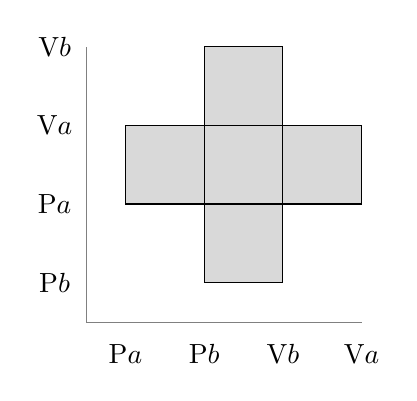
\begin{tikzpicture}[-]
    \path (.5,.5) edge[gray] (4,.5);
    \path (.5,.5) edge[gray] (.5,4);
    \draw[fill=gray!30] (1,2) -- (4,2) -- (4,3) -- (1,3) -- (1,2);
    \draw[fill=gray!30] (2,1) -- (2,4) -- (3,4) -- (3,1) -- (2,1);
    \draw (2,2) -- (3,2) -- (3,3) -- (2,3) -- (2,2);
    \node at (1,.1) {P$a$};
    \node at (2,.1) {P$b$};
    \node at (3,.1) {V$b$};
    \node at (4,.1) {V$a$};
    \node at (.1,1) {P$b$};
    \node at (.1,2) {P$a$};
    \node at (.1,3) {V$a$};
    \node at (.1,4) {V$b$};
  \end{tikzpicture}
\end{document}